El Nivel Regulatorio constituye el sistema de control en tiempo real del robot. Su responsabilidad principal es la gestión directa de actuadores (motores paso a paso, servomotores, gripper) y sensores (finales de carrera), ejecutando comandos de movimiento con precisión temporal estricta.

El firmware se estructura en tres capas jerárquicas que separan las responsabilidades según el nivel de abstracción (Figura \ref{fig:arquitectura_regulatorio}):

\textbf{Capa de Controladores de Hardware}: Interactúa directamente con los periféricos del microcontrolador mediante registros y temporizadores. Incluye el controlador de motores paso a paso que genera pulsos mediante el Timer1, el controlador de servomotores que utiliza PWM por hardware con Timer4 y Timer5, el controlador del actuador de agarre que maneja el motor paso a paso, y el controlador de comunicación serial que implementa buffers circulares manejados por interrupciones.

\textbf{Capa de Control de Movimiento}: Implementa algoritmos de generación de trayectorias y perfiles de velocidad. El generador de perfiles trapezoidales calcula las velocidades instantáneas en cada fase del movimiento, el gestor de límites supervisa los finales de carrera y detiene los ejes cuando es necesario, y el coordinador de movimientos sincroniza múltiples ejes para trayectorias rectilíneas.

\textbf{Capa de Aplicación}: Proporciona la interfaz de alto nivel para comandos del sistema supervisor. El intérprete de comandos procesa las instrucciones recibidas por UART y las traduce en acciones de control, el protocolo de comunicación define el formato de mensajes y respuestas, y el módulo de configuración centraliza parámetros como velocidades máximas, aceleraciones y límites de seguridad.

\begin{figure}[H]
    \centering
    % TODO: Insertar diagrama de capas del firmware regulatorio
    % Mostrar: Aplicación → Control → Drivers → Hardware
    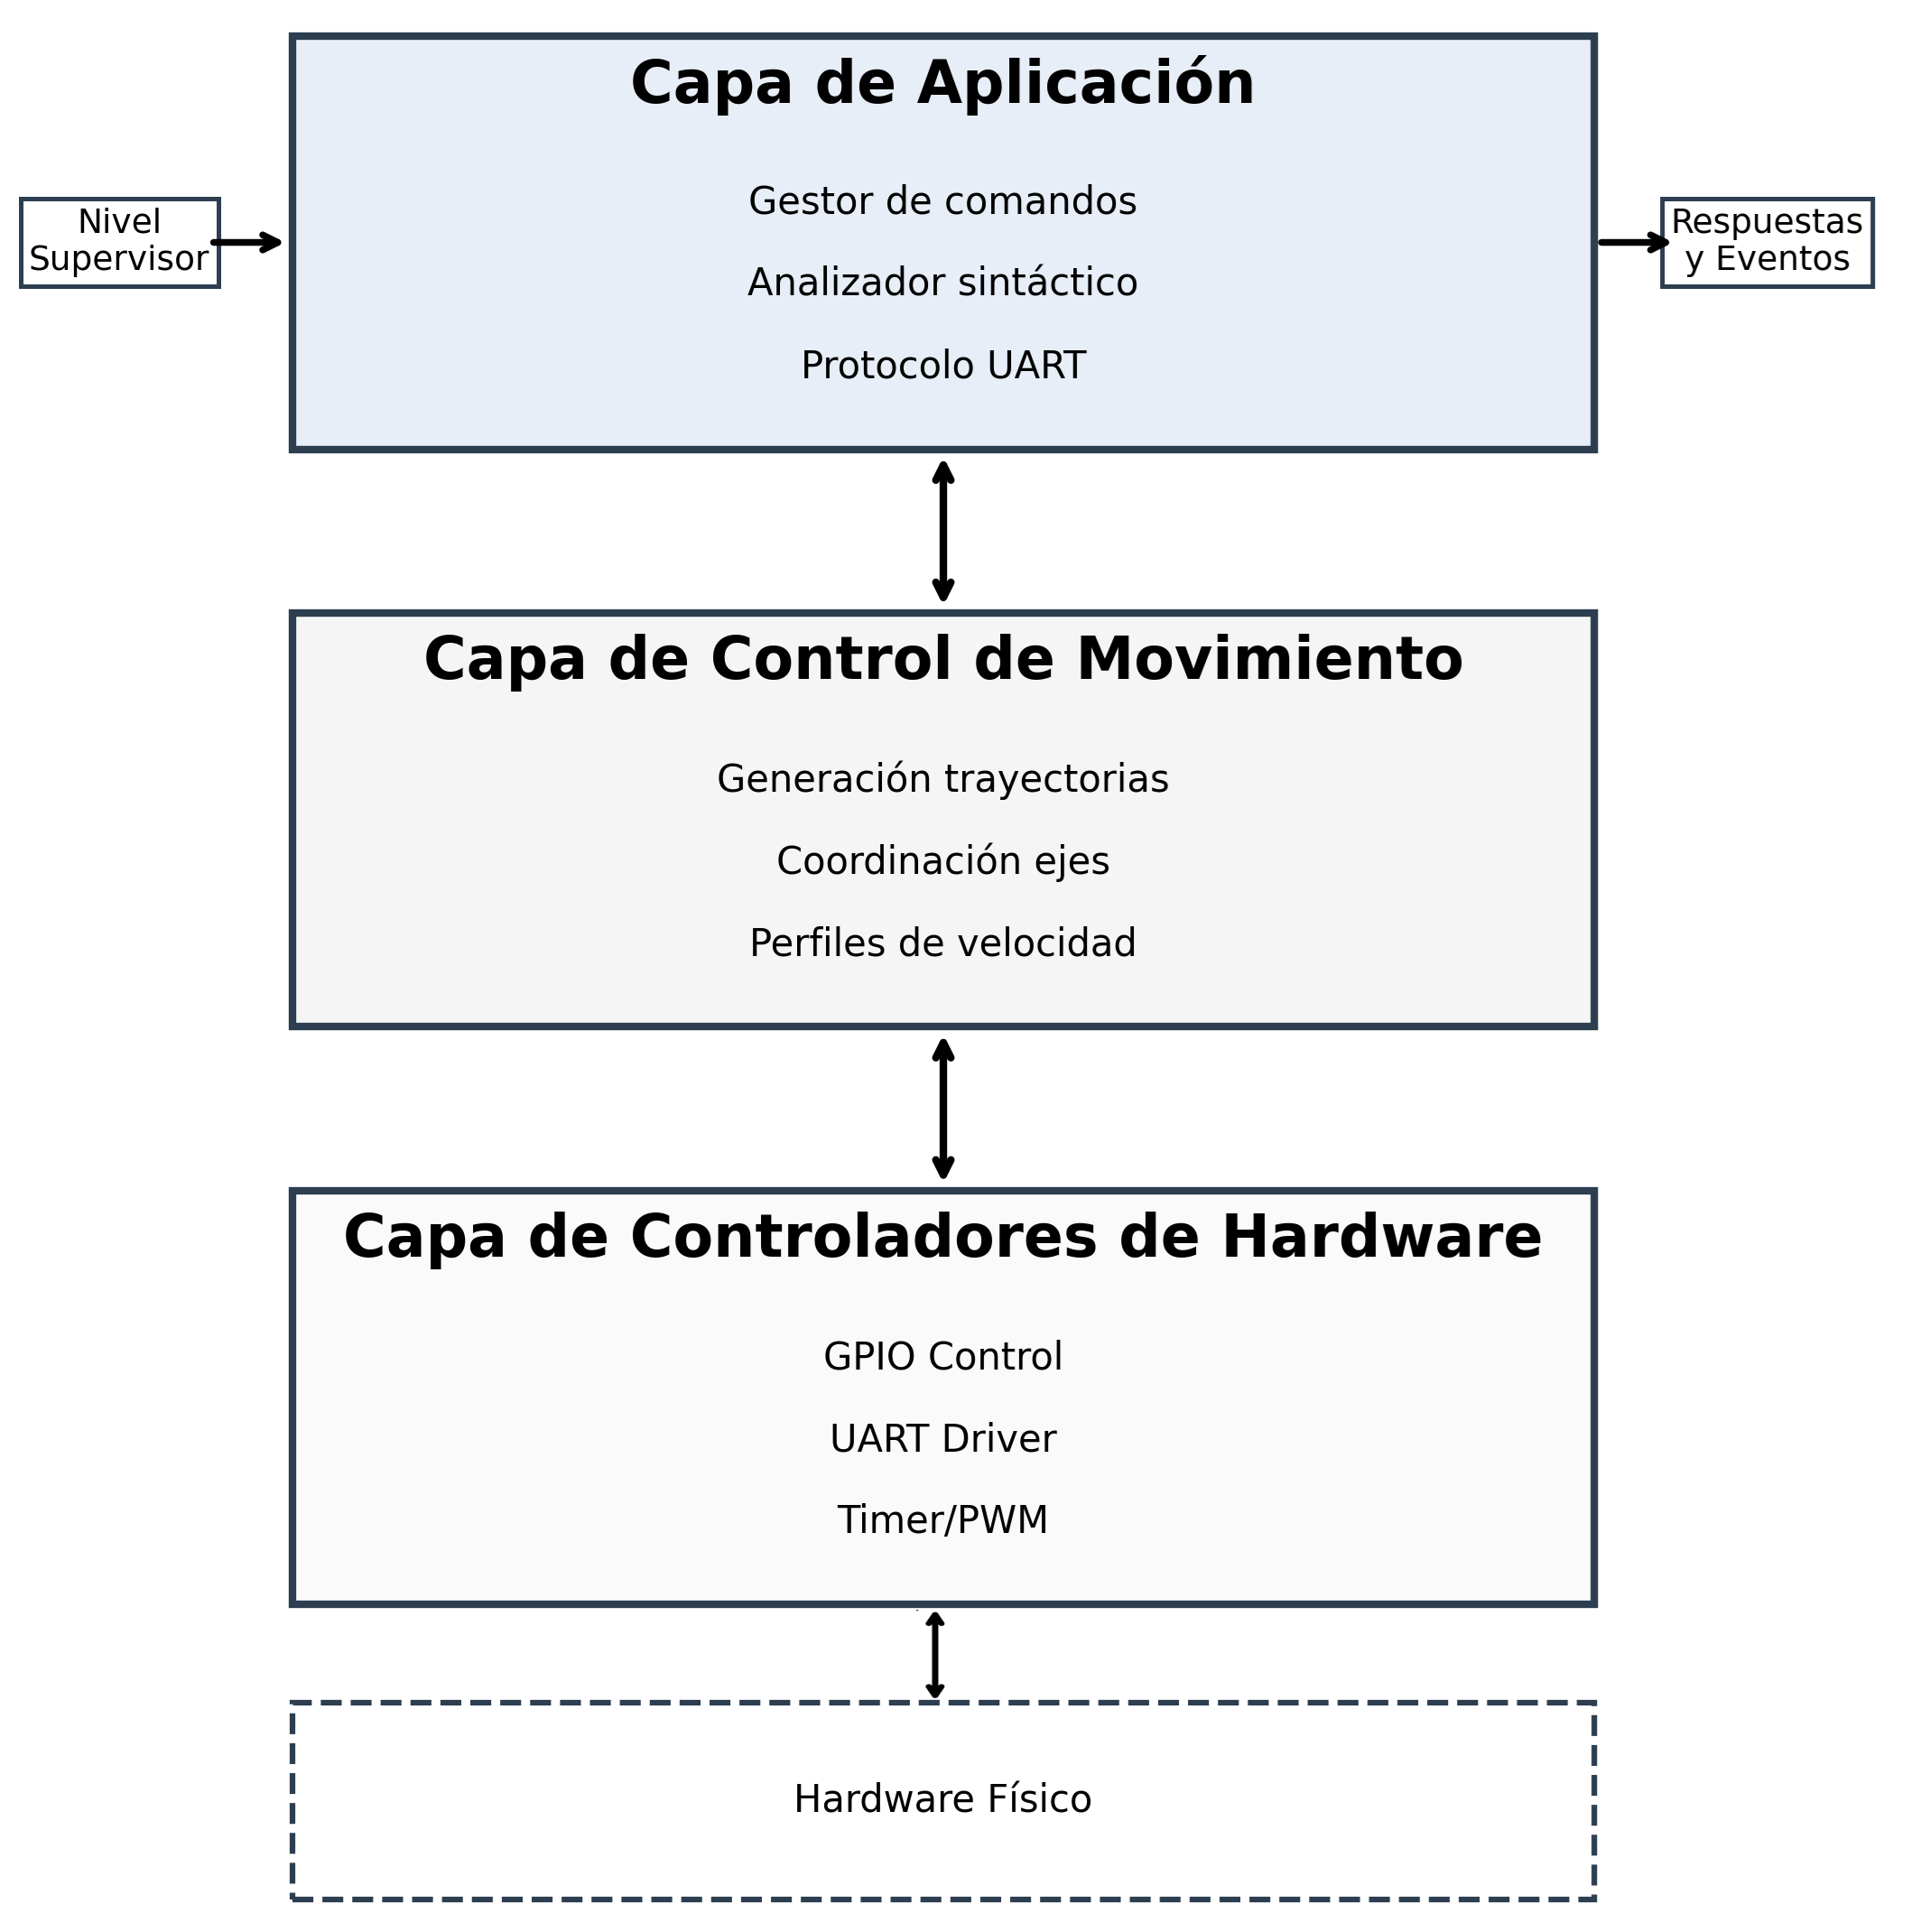
\includegraphics[width=0.6\textwidth]{imagenes/arquitectura_regulatorio_capas.png}
    \caption{Arquitectura en capas del firmware del Nivel Regulatorio}
    \label{fig:arquitectura_regulatorio}
\end{figure}

Esta arquitectura permite que el nivel regulatorio ejecute movimientos coordinados con precisión mientras mantiene comunicación bidireccional fluida con el supervisor.
